\section{Rasa: Open Source Language Understanding and Dialogue Management \cite{bocklisch2017}}
\label{sec:bocklisch2017}

No campo de estudo da interação humano-computador, há uma procura por formas mais naturais de adicionar automações na vida cotidiana. Nesse contexto, é bastante difundido o uso de sistemas conversacionais, e dentre alguns dos mais conhecidos estão a Siri da Apple, a Alexa da Amazon e a Cortana da Microsoft.

No artigo de \citeonline{bocklisch2017}, são apresentadas as ferramentas Rasa NLU e Rasa Core, que são bibliotecas de código aberto para a linguagem Python focadas, respectivamente, em processamento de linguagem natural e gerenciamento de diálogo. O intuito é facilitar a construção de sistemas conversacionais, com gerenciamento de diálogo baseado em aprendizado de máquina e processamento de linguagem natural, para desenvolvedores que não precisam ser necessariamente especialistas nessas áreas.

A API do Rasa utiliza ideias implementadas em outras bibliotecas de aprendizado de máquina, como herança estrita do \textit{scikit-learn} \apud{bocklisch2017}{chollet2015} e diferentes implementações de back-end do \textit{Keras} \apud{bocklisch2017}{pedregosa2011}.

A classificação de textos é vagamente baseada na abordagem \textit{fastText} \apud{bocklisch2017}{joulin2016}. As sentenças são representadas pelo agrupamento de vetores de palavras para cada token constituinte. Usando \textit{embeddings} (representações de valores ou objetos projetados para serem consumidos por modelos de aprendizado de máquina) de palavras pré-treinadas como \textit{GloVe} \apud{bocklisch2017}{pennington2014}, os classificadores de intenção são notavelmente mais robustos às variações da linguagem do que quando treinados com apenas alguns exemplos de cada intenção.

O Rasa é projetado com uma arquitetura modular. Desse modo, é possível integrá-lo facilmente com outros sistemas. Por exemplo, o Rasa Core pode ser usado como um gerenciador de diálogos em conjunto com outros serviços de NLU que não sejam o Rasa NLU. Embora eles sejam implementados em Python, ambos os serviços podem ser expostos via rede, permitindo a utilização deles em projetos feitos em outras linguagens de programação.

Na Figura \ref{fig:architecture-rasa}, é demonstrada graficamente a série de passos feitos pelo Rasa quando uma nova mensagem é recebida. Vale ressaltar que o passo 1 é feito pelo Rasa NLU, enquanto os demais são realizados pelo Rasa Core. No passo 1, a mensagem é recebida e passada para um interpretador (por exemplo, Rasa NLU) para extrair a intenção, entidades e qualquer outra informação estruturada. No passo 2, o \textit{Tracker} é notificado que uma nova mensagem foi recebida, e armazena o estado da conversa em um banco de dados. Nos passos 3 e 4, o estado atual da conversa é passado para o objeto \textit{Policy}, que será responsável por escolher a próxima ação. No passo 5, a ação escolhida é registrada no \textit{Tracker}. No passo 6, a ação é executada.

\begin{figure}[ht] 
   	\captionsetup{width=16cm}
	\Caption{\label{fig:architecture-rasa} Arquitetura do Rasa}
	\UFCfig{}{
        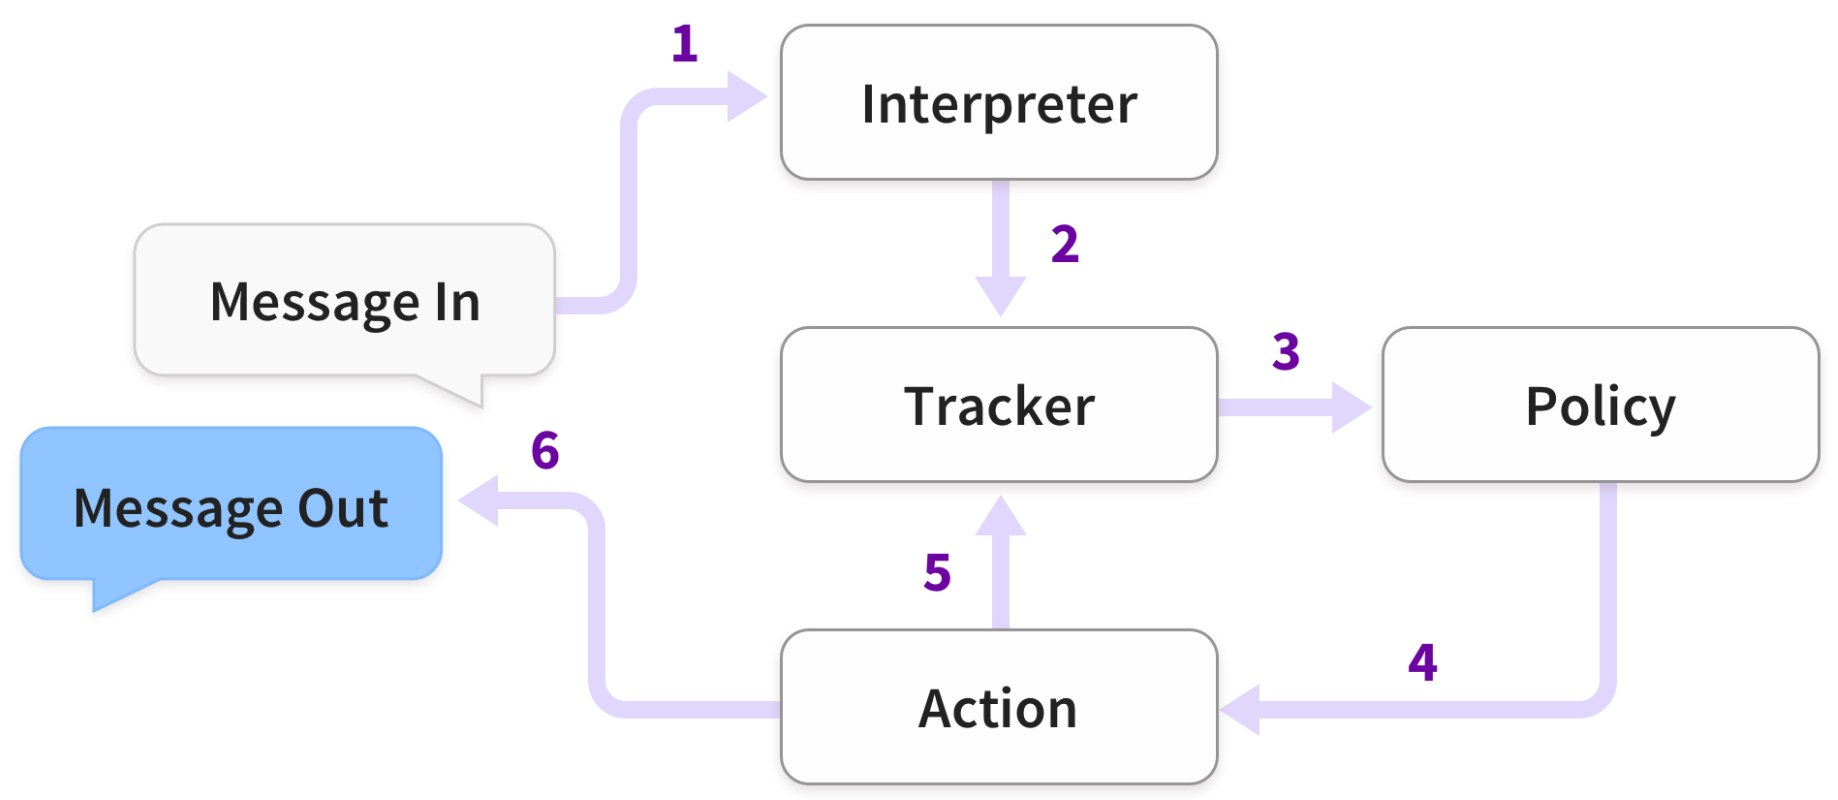
\includegraphics[width=16cm]{figuras/architecture-rasa.png}
    }{
		\Fonte{\citeonline{bocklisch2017}.}
	}
\end{figure}

O estado do diálogo é persistido em um objeto \textit{Tracker}, sendo ele único por seção de conversa. Além disso, ele é o único componente do sistema que possui estado. O \textit{Tracker} registra todos os eventos que levaram a aquele estado e que ocorreram durante a conversa. O estado da conversa pode ser reconstruído a partir desses eventos.

No Rasa, o problema de gerenciamento de diálogo é tratado como um problema de classificação. A cada iteração, o Rasa Core prevê qual será a próxima ação a ser tomada com base em uma lista predefinida de ações. Uma ação pode ir desde uma mensagem a ser enviada para o usuário até a execução de uma função arbitrária. Na execução da ação, é passada uma instância do objeto \textit{Tracker} da sessão, permitindo assim que a ação tenha acesso a qualquer informação relevante coletada previamente no diálogo.

Em adição ao aprendizado supervisionado, o Rasa Core fornece uma abordagem que permite que os desenvolvedores apliquem correções durante o seu treinamento, como exemplificado na Figura \ref{fig:rasa-training-correction}, em que após o usuário fornecer a entrada ``/greet'' destacada em verde, o Rasa Core escolheu a ação ``utter\_ask\_howcanhelp'' destacada em vermelho, e questionou se essa ação era correta com base na entrada. Caso seja informado que a ação é incorreta, será mostrada a lista de possíveis ações, bem como cada probabilidade associada a elas pelas políticas da conversa (Figura \ref{fig:rasa-actions}).

\begin{figure}[ht] 
   	\captionsetup{width=16cm}
	\Caption{\label{fig:rasa-training-correction} Exemplo de correção durante o treinamento do Rasa}
	\UFCfig{}{
        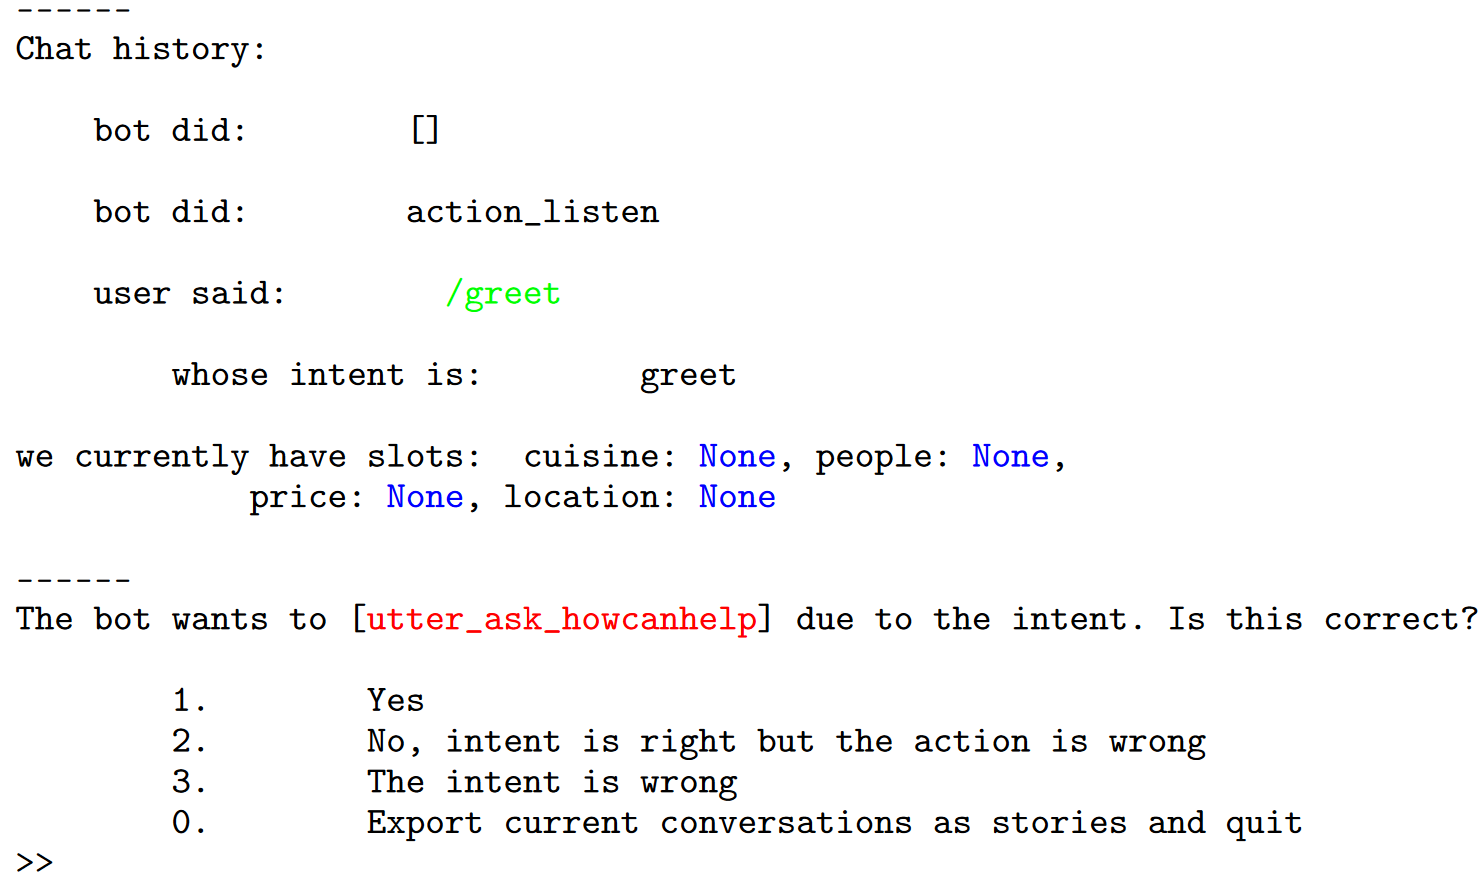
\includegraphics[width=16cm]{figuras/rasa-training-correction.png}
    }{
		\Fonte{\citeonline{bocklisch2017}.}
	}
\end{figure}

\begin{figure}[ht] 
   	\captionsetup{width=16cm}
	\Caption{\label{fig:rasa-actions} Exemplo de escolha da próxima ação do Rasa durante a correção}
	\UFCfig{}{
        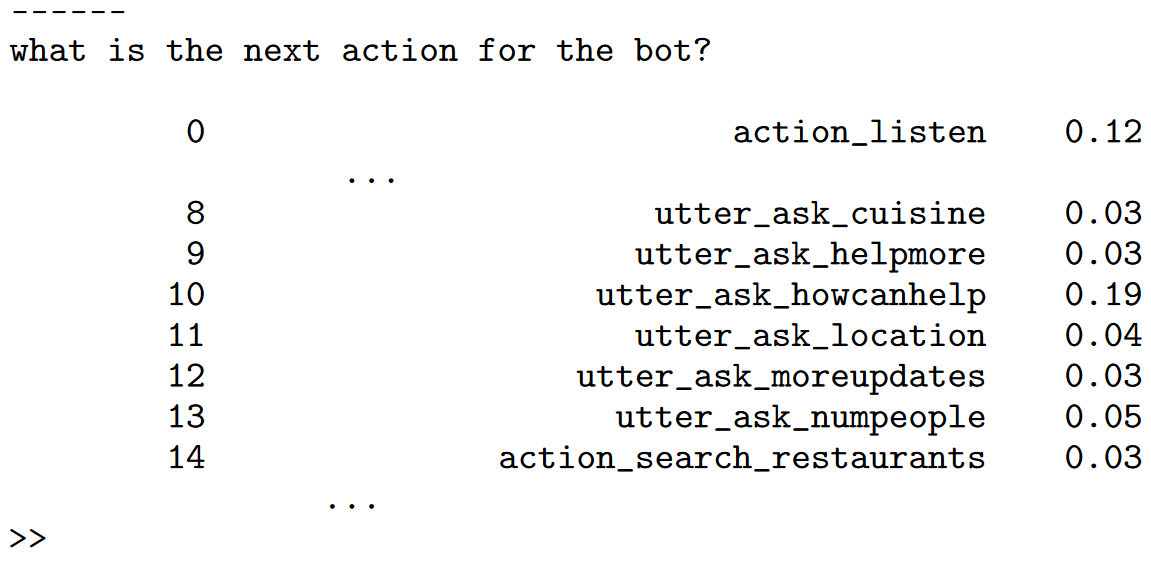
\includegraphics[width=16cm]{figuras/rasa-actions.png}
    }{
		\Fonte{\citeonline{bocklisch2017}.}
	}
\end{figure}

Tanto o Rasa NLU quanto o Rasa Core estão sendo desenvolvidos ativamente. Eles são plataformas gratuitas para a aplicação de pesquisas em modelos conversacionais de inteligência artificial por desenvolvedores que não precisam ser especialistas nessas áreas, e portanto não há previsão de serem finalizados.